%------------------------------------------%
% Cannabis Data Science
% Date: 3/16/2022
%------------------------------------------%
\documentclass[xcolor={dvipsnames}]{beamer}
\hypersetup{pdfpagemode = FullScreen}
\mode<presentation>{
  \usetheme{Boadilla}
  \usecolortheme{orchid}
  \usefonttheme{default}
  \setbeamertemplate{navigation symbols}{}
  \setbeamertemplate{caption}[numbered]
}
\setbeamersize{
  text margin left = 0.5in,
  text margin right = 0.5in
}

%------------------------------------------%
% Title
%------------------------------------------%
\title[\textbf{Cannabis Data Science \#57}]{}
\author{Cannabis Data Science}
\institute[]{\Large Cannabis Data Science \#57}
\date{March \nth{16}, 2022}

%------------------------------------------%
% Packages
%------------------------------------------%
\usepackage[english]{babel}
\usepackage[utf8x]{inputenc}
\usepackage{tikz} % For styling.
\usepackage{xparse}

%------------------------------------------%
% Colors
%------------------------------------------%
\definecolor{Green}{RGB}{34, 153, 84}
\definecolor{LightGreen}{RGB}{218, 247, 166}
\definecolor{DarkGreen}{RGB}{2, 48, 32}
\definecolor{Orange}{RGB}{255, 87, 51}
\definecolor{DarkOrange}{RGB}{199, 0, 57}
\definecolor{Yellow}{RGB}{255, 195, 0}

%------------------------------------------%
% Theme
%------------------------------------------%
\setbeamercolor*{palette primary}{bg=LightGreen, fg=DarkGreen}
\setbeamercolor*{palette secondary}{bg=LightGreen, fg=DarkGreen}
\setbeamercolor*{palette tertiary}{bg=LightGreen, fg=DarkGreen}

%------------------------------------------%
% Packages
%------------------------------------------%
\usepackage{amsmath}
\renewcommand*\footnoterule{} % No separating line on footnote.
\usepackage{mathtools} % For annotating equations.
\usepackage{hhline} % for double bars.
\usepackage[super]{nth} % For formatting 1st, 2nd, 3rd, etc.
\usepackage{graphicx, caption, subcaption}

%------------------------------------------%
% Commands
%------------------------------------------%

% Top space.
\newcommand\T{\rule{0pt}{2.5ex}}

% Bottom space.
\newcommand\B{\rule[-1.25ex]{0pt}{0pt}}

% Blocks.
\newenvironment<>{Block}[2][.9\textwidth]
  {\setlength{\textwidth}{#1}
  \begin{actionenv}#3
    \def\insertblocktitle{#2}\par
    \usebeamertemplate{block begin}}
  {\par\usebeamertemplate{block end}
  \end{actionenv}}

% Balls.
\defbeamertemplate{enumerate item}{largeball}
{\begin{pgfpicture}{-1ex}{-0.65ex}{1.5ex}{1.5ex}
\usebeamercolor[fg]{item projected}
{\pgftransformscale{2.5}\pgftext{\Large\pgfuseshading{bigsphere}}}
{\pgftransformshift{\pgfpoint{0pt}{0.5pt}}
\pgftext{\usebeamerfont*{item projected}\small\insertenumlabel}}
\end{pgfpicture}}

% Fancy arrows.
\NewDocumentCommand\UpArrow{O{2.0ex} O{black}}{%
   \mathrel{\tikz[baseline] \draw [->, line width=0.5pt, #2] (0,0) -- ++(0,#1);}} % Fancy up-arrow.
\NewDocumentCommand\DownArrow{O{2.0ex} O{black}}{%
   \mathrel{\tikz[baseline] \draw [<-, line width=0.5pt, #2] (0,0) -- ++(0,#1);}} % Fancy down-arrow.

% Equations with numbers on the left.
\makeatletter
\newcommand{\LeftEqNo}{\let\veqno\@@leqno}
\makeatother

%------------------------------------------%
% Presentation
%------------------------------------------%
\begin{document}

% Title page.
\begin{frame}{}
  
\includegraphics[scale=0.33]{images/logo.pdf}
  \vspace*{-2\baselineskip}
  \titlepage

  % TODO: Add flare to title page?
  % Background
%\tikz[remember picture, overlay]
%\node[opacity=1.0, inner sep=0pt] at (current page.center){
%  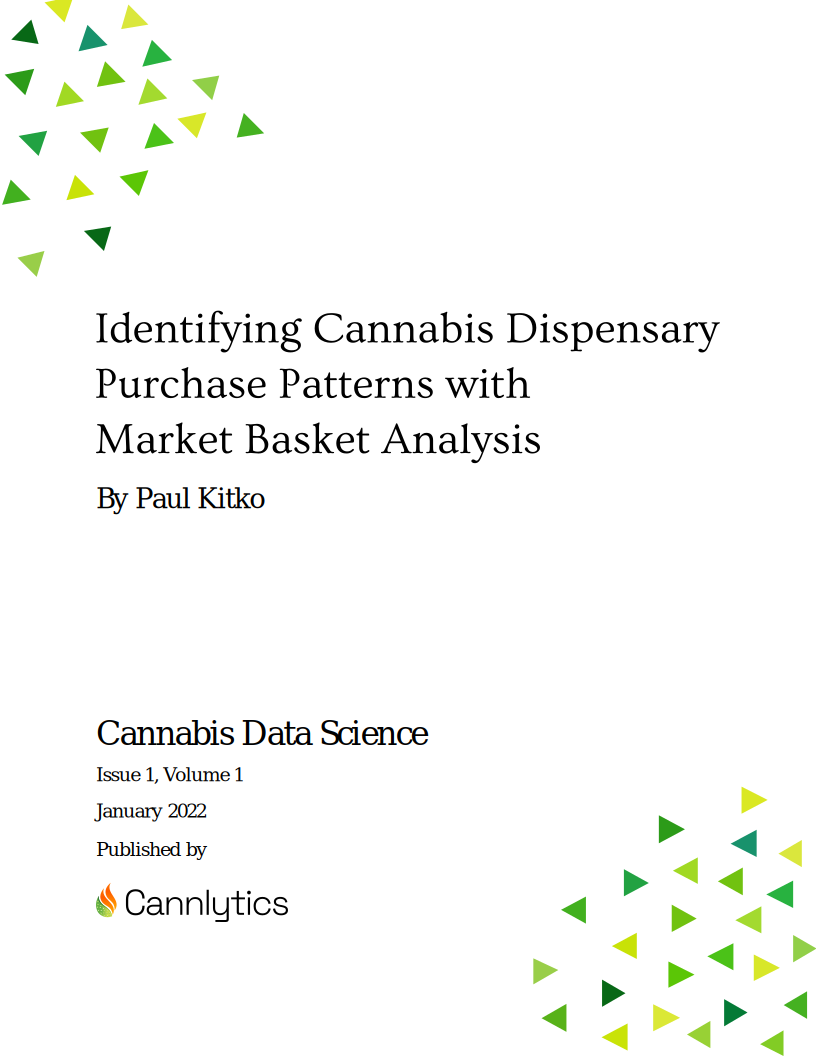
\includegraphics[width=\paperwidth, height=\paperheight]{images/cover.pdf}
%};  
  
\end{frame}

%------------------------------------------%
% Data Science
%------------------------------------------%
\section{Data Science}

\begin{frame}{What Data Science Brings to the Table}

\vspace*{0.125\baselineskip}

\begin{figure}
\includegraphics[height=1.5in]{images/winds-of-britain.png}
\caption*{%
  \tiny Daily wind patterns of Britain mapped by Francis Galton, {\itshape Meteorographica} (1863).
 }
\end{figure}

\begin{center}
\begin{minipage}{0.8\textwidth}
{\footnotesize\itshape ``...by \underline{drawing diagrams}, and \underline{by countings}. This much suffices to give a correct idea of the {\bfseries distribution} of any given set of variables ; it is also sufficient to give a fair idea of the closeness of {\bfseries correlation}, or of kinship, between any two sets of variables.''}
\end{minipage}
\end{center}

%\vspace*{0.05\baselineskip}

\begin{flushright}
\begin{minipage}{0.6\textwidth}
{\footnotesize -- {\bfseries Francis Galton} in a letter to the editor of {\itshape The Times} on {\itshape Alcoholism and Offspring}.}
\end{minipage}
\end{flushright}

%Measurements vary.

\end{frame}


%------------------------------------------%
% Background
%------------------------------------------%
\section{Background}

\begin{frame}{An Odd History of Data Exploration}

\vspace*{0.5\baselineskip}

Sir Francis Galton opened an anthropometric laboratory to

\vspace*{0.25\baselineskip}

\begin{center}
\begin{minipage}{0.8\textwidth}
{\footnotesize\itshape ``show the public the \underline{simplicity} of the instruments and methods by which the chief physical characteristics of man may be \underline{measured} and \underline{recorded}.''}
\end{minipage}
\end{center}

\vspace*{0.25\baselineskip}

\begin{center}
\begin{minipage}{0.45\textwidth}

\begin{figure}
\includegraphics[height=1.8in]{images/sir-francis-galton-1850s.jpg}
\caption*{%
  \tiny Sir Francis Galton (1822 – 1911) in the 1850s.\\
 }
\end{figure}

\end{minipage}\hspace{0.05\textwidth}%
\begin{minipage}{0.45\textwidth}


\begin{figure}
\includegraphics[height=1.8in]{images/anthro-lab-poster.jpg}
\caption*{%
  \tiny Flyer advertising the Anthropometric Laboratory.\\
 }
\end{figure}

\end{minipage}
\end{center}


\end{frame}

%------------------------------------------%
% Francis Galton
%------------------------------------------%

\begin{frame}{Francis Galton's Fingerprint on Data Science}

\begin{minipage}{0.45\textwidth}

\begin{itemize}
\item Penchant for \underline{counting} and \underline{measuring}.

\vspace*{0.25\baselineskip}

\item Founded the biometric approach to the study of heredity.

\vspace*{0.25\baselineskip}

\item Taught and founded {\itshape Biometrika} with Karl Pearson.

\vspace*{0.25\baselineskip}

\item Introduced the concepts:

\begin{itemize}
\item {\bfseries standard deviation};
\item {\bfseries correlation};
\item {\bfseries regressions}.
\end{itemize}
  
\end{itemize}


\end{minipage}\hspace{0.05\textwidth}%
\begin{minipage}{0.45\textwidth}

\begin{figure}
\includegraphics[height=1.5in]{images/distribution-of-successful-men.png}
\caption*{%
  \tiny Distribution of Successes and of Natural Ability Among the Kinsfolk of Fellows of the Royal Society (1904).\\
 }
\end{figure}

\end{minipage}

\end{frame}

%------------------------------------------%
% Francis Galton's work
%------------------------------------------%

\begin{frame}{Francis Galton's Work}

\begin{figure}
\includegraphics[height=2in]{images/rate-of-regression.png}
\caption*{%
  \tiny An application of regression and prediction by Francis Galton in {\itshape Anthropological Miscellanea} (1886).\\
 }
\end{figure}

\begin{itemize}

\item Created a dataset of 9,337 respondents, each measured in 17 categories.

\item After applying the \underline{liner regression} to sweat peas, Francis Galton applied regressions to the human data.

\end{itemize}

\end{frame}

%------------------------------------------%
% FIXME: Introduction
%------------------------------------------%
%\section{Introduction}
%
%\begin{frame}{}
%
%\begin{minipage}{0.7\textwidth}
%
%\vspace{-2\baselineskip}
%
%% Question of the day
%\begin{center}
%\begin{minipage}{.9\linewidth}
%\begin{Block}{Question of the day}
%
%\vspace{.5\baselineskip}
%\begin{itemize}
%\item What insights does our data hold that we may not know?
%\end{itemize}
%
%\vspace{.5\baselineskip}
%
%\end{Block}
%\end{minipage}
%\end{center}
%
%\end{minipage}\hspace{0.05\textwidth}%
%%\begin{minipage}{0.25\textwidth}
%%
%%\vspace{0.5\baselineskip}
%%
%%\end{minipage}
%
%\end{frame}

%------------------------------------------%
% Exploratory Data Analysis
%------------------------------------------%

\begin{frame}{An aside on studying}

{\itshape Weekly Evening Meeting} By Francis Galton

{\itshape On Men of Science, their Nature and their Nurture}

\vspace{0.75\baselineskip}

\begin{itemize}

\item \underline{Not tied down} to old courses of classics and mathematics.

\vspace{.5\baselineskip}

\item Sufficient groundwork in many subjects to avoid error.

\vspace{.5\baselineskip}

\item Early introduced to \underline{many subjects} of interest.

\vspace{.5\baselineskip}

\item A well--balanced education, including {\bfseries chemistry}, {\bfseries botany}, {\bfseries logic}, and {\bfseries political economy}.

\vspace{.5\baselineskip}

\item A variety of subjects, and \underline{attention to details}.

\vspace{.5\baselineskip}

\item Coming in contact with persons of every rank and sitting in the same form.

\end{itemize}

\end{frame}

%------------------------------------------%
% Takeaway
%------------------------------------------%
\section{Takeaway}
\begin{frame}{}

\begin{center}
\begin{minipage}{3.85in}

% Thank you.
\includegraphics[width=.25in]{images/prayer.png} {\Large \textbf{Thank you for coming.}}\\

\begin{center}
\begin{minipage}{.9\linewidth}
\begin{Block}{Lessons of the Day}

\vspace{0.5\baselineskip}

\begin{itemize}

\item Measurements vary.

\vspace{0.5\baselineskip}

\item Exploring your data is an critical, yet often overlooked, step in gleaming insights.

\vspace{0.5\baselineskip}

\end{itemize}

\end{Block}
\end{minipage}
\end{center}

\vfill

\end{minipage}
\end{center}

\end{frame}

%------------------------------------------%
% Fin.
%------------------------------------------%
\end{document}
